\subsection{K Nearest Neighbors classification}\label{sec:kNN}
Our next choice is \emph{k Nearest Neighbors} (kNN), as it is a common and intuitive classification method. 

\subsubsection{Classification method}
To describe the classification, we divide it into two steps. Like all classifiers of scikit-learn, first we \emph{fit} the model with training data, then we \emph{predict} the labels of our test data.

Other than most models, a kNN-classifier is fitted by simply projecting the $n$-dimensional data in an $n$-dimensional feature space. The computation heavy step is the prediction. The probability of a data point from the test set is estimated by a simple vote of the \emph{k} nearest neighbors. The proximity of a point to this test data point is measured in their \emph{Euclidian distance}. We create Fig. \ref{fig:knn} to visualize the prediction method of kNN. By choosing odd-numbered \emph{k}, we avoid possible even vote results.

\begin{figure}[h]
	\centering
	\begin{subfigure}[t]{0.48\textwidth}
		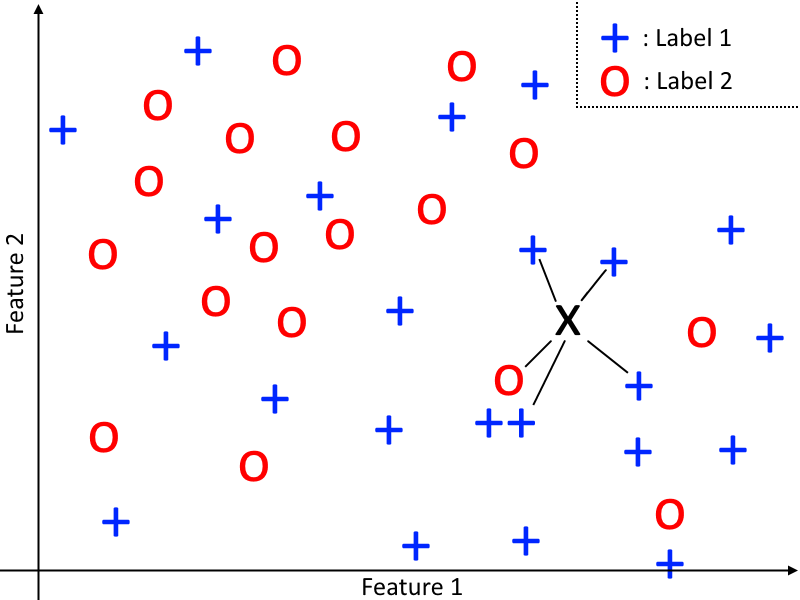
\includegraphics[width=\textwidth]{images/knn1}
        \caption{Insert new datapoint and find k (here =5) nearest neighbors.}
	\end{subfigure}
	\quad
	\begin{subfigure}[t]{0.48\textwidth}
		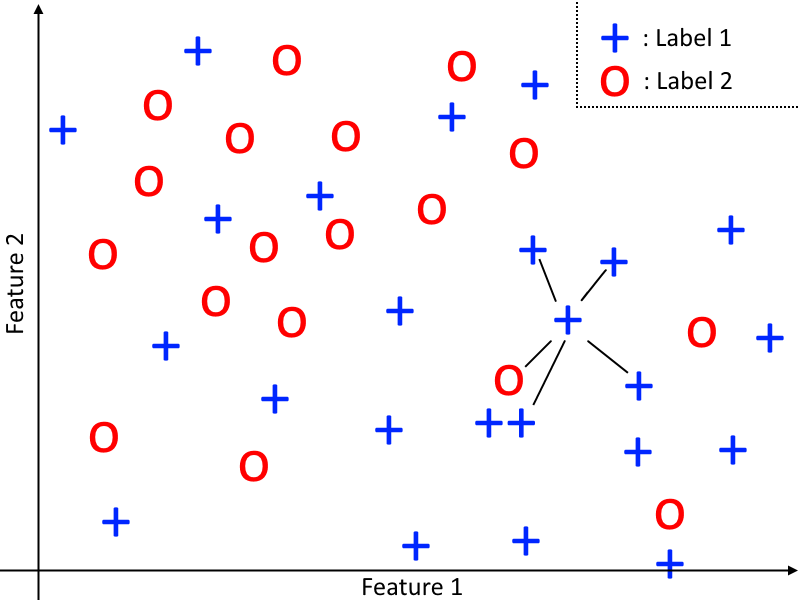
\includegraphics[width=\textwidth]{images/knn2}
        \caption{Predict datapoints label by majority vote.}
	\end{subfigure}
	\caption{Visualization of kNN-classification with k=5}
	\label{fig:knn}
\end{figure}


\subsubsection{Performance and optimization}
Compared to logistic regression, kNN achieves with default parameters and the complete data a much higher AMS. We can improve our score mainly with changing two parameters. The first option is to use feature selection on our data, as kNN is highly influenced by this choice. This also improves the runtime of the classifier, as the calculation of distances between vectors increases with their dimensionality. For testing these selections, low \emph{k} like 10 or 20 are sufficient. After we find a good feature set, tuning \emph{k} is the second parameter kNN mainly relies on. Larger \emph{k} suppresses noise, but softens the classification boundaries and increases runtime. The sets we created with help of kNN ensembles result in worse scores than our hand-crafted sets. We achieve the best public AMS with feature set 6 and \emph{k} = 297 after 123.67 seconds prediction time. The relation of \emph{k}, prediction time and the resulting public AMS is presented by Fig. \ref{fig:knnams} and \ref{fig:knnspeed}, which uses data we recorded during testing.

\begin{figure}
	\centering
	\begin{subfigure}[b]{0.49\textwidth}
		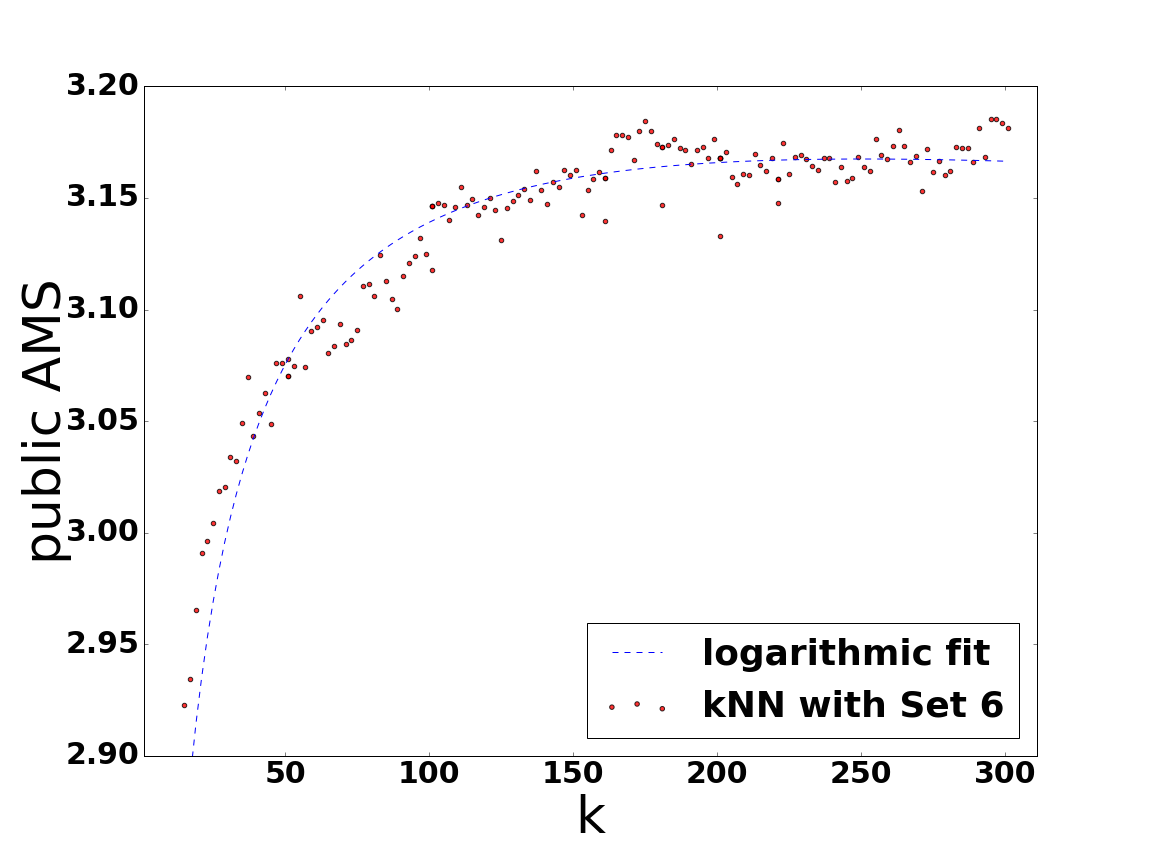
\includegraphics[trim=0 0 0 20,clip,width=\textwidth]{images/knn_ams}
        \caption{kNN results on Set 6}
        \label{fig:knnams}
	\end{subfigure}
	\begin{subfigure}[b]{0.49\textwidth}
		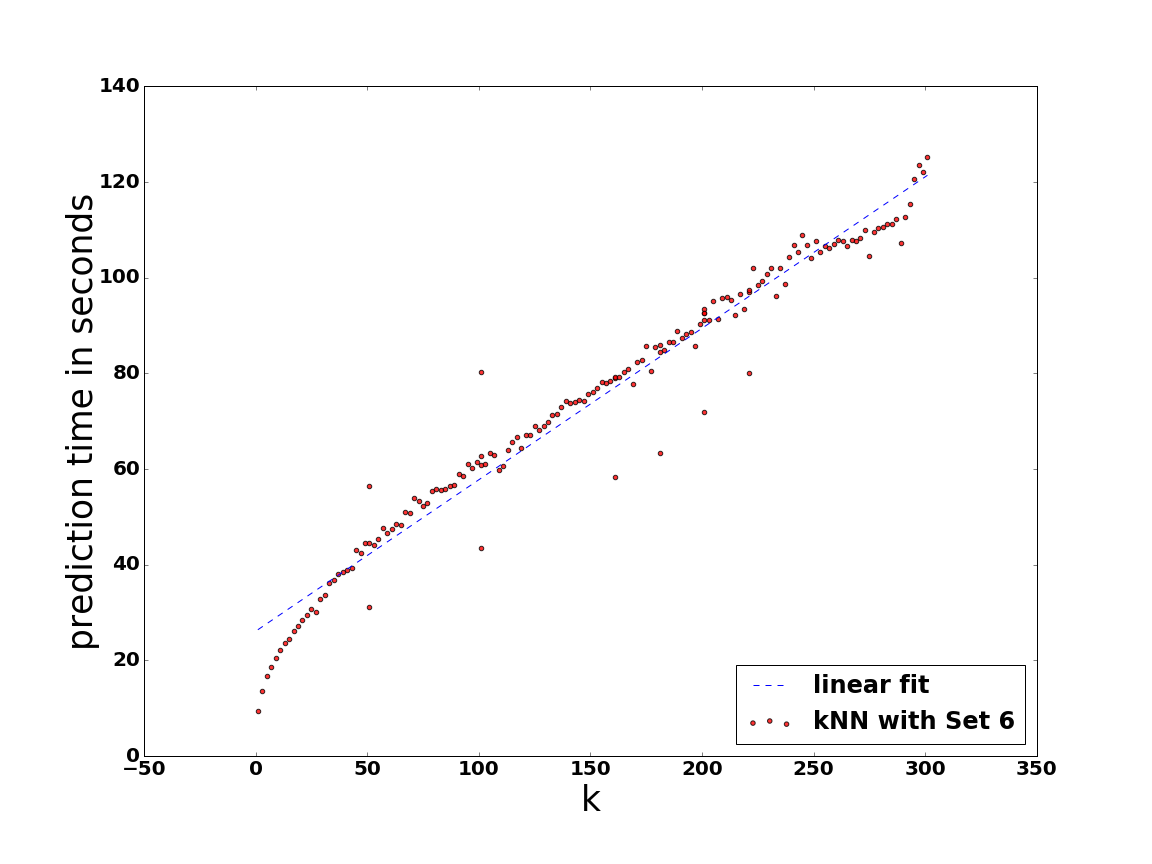
\includegraphics[trim=20 0 0 0,clip,width=\textwidth]{images/knn_speed}
        \caption{kNN prediction time on Set 6}
        \label{fig:knnspeed}
	\end{subfigure}
	\caption{kNN performance on feature set 6}
	\label{fig:knn_perf}
\end{figure}

Our results surpass those by another team that uses kNN. They identify the replacement of missing data values by the features mean as main error \cite{california}. Considering that our optimal feature sets (Tab. \ref{tab:feats}) contain none of \texttt{PRI\_jet\_num}-related data, except \texttt{PRI\_jet\_num} itself, support this assumption.